\documentclass[10pt,a4paper]{article}

% --- Packages & Geometry ---
\usepackage[utf8]{inputenc}
\usepackage[T1]{fontenc}
\usepackage[margin=0.8in,headheight=14pt,headsep=16pt,footskip=20pt]{geometry}
\usepackage{lmodern}
\usepackage{microtype}
\usepackage{xcolor}
\usepackage{graphicx}
\usepackage{amsmath,amssymb}
\usepackage{booktabs}
\usepackage{array}
\usepackage{tabularx}
\usepackage{enumitem}
\usepackage{fancyhdr}
\usepackage{tcolorbox}
\usepackage{float}
\usepackage{tikz}
\usetikzlibrary{shapes.geometric, arrows.meta, positioning, calc, backgrounds, fit}

% --- Hyperref Setup ---
\usepackage{hyperref}
\hypersetup{
    colorlinks=true,
    linkcolor=deepblue,
    citecolor=deepblue,
    urlcolor=accentblue,
    pdfauthor={Risan Raja (DA25G521)},
    pdftitle={MLOps Pipeline with Docker and Kubernetes - Technical Report},
    pdfsubject={MLOps PyTorch Pipeline Assignment Report}
}

% --- Color Palette ---
\definecolor{primarydark}{HTML}{0F172A}   % Deep Slate / Navy
\definecolor{deepblue}{HTML}{1E40AF}      % Corporate Blue
\definecolor{accentblue}{HTML}{2563EB}    % Vibrant Blue
\definecolor{softblue}{HTML}{EFF6FF}      % Light Blue Background
\definecolor{borderblue}{HTML}{BFDBFE}    % Border Blue
\definecolor{cardbg}{HTML}{F8FAFC}        % Card Background
\definecolor{codebg}{HTML}{F1F5F9}        % Code snippet background
\definecolor{darkgray}{HTML}{334155}      % Body Dark Gray
\definecolor{lightgray}{HTML}{64748B}     % Subdued Gray
\definecolor{taggreen}{HTML}{16A34A}      % Success Green
\definecolor{tagblue}{HTML}{0284C7}       % Info Blue

% --- TColorBox Styling ---
\tcbuselibrary{skins,breakable}

\newtcolorbox{metadatabox}{
    colback=softblue,
    colframe=borderblue,
    arc=3mm,
    boxrule=0.9pt,
    left=10pt, right=10pt, top=7pt, bottom=7pt,
    enhanced,
    drop shadow=black!5!white
}

\newtcolorbox{reflectionbox}[1]{
    colback=cardbg,
    colframe=deepblue,
    arc=2.5mm,
    boxrule=0.8pt,
    title={\textbf{#1}},
    coltitle=white,
    colbacktitle=deepblue,
    left=9pt, right=9pt, top=7pt, bottom=7pt,
    enhanced
}

% --- Header & Footer Configuration ---
\pagestyle{fancy}
\fancyhf{}
\fancyhead[L]{\textcolor{lightgray}{\footnotesize\textbf{MLOps PyTorch Pipeline} $\cdot$ Assignment Technical Report}}
\fancyhead[R]{\textcolor{lightgray}{\footnotesize\textbf{Risan Raja} (Roll: DA25G521)}}
\fancyfoot[C]{\textcolor{lightgray}{\footnotesize Page \thepage\ of 2}}
\renewcommand{\headrulewidth}{0.4pt}
\renewcommand{\footrulewidth}{0.4pt}

% --- Paragraph & List Spacing ---
\setlength{\parindent}{0pt}
\setlength{\parskip}{4.5pt}
\setlist{topsep=1.5pt, itemsep=1.8pt, parsep=1.2pt}

% ==============================================================================
% DOCUMENT BODY
% ==============================================================================
\begin{document}

% --- Title & Metadata Banner ---
\begin{center}
    {\fontsize{16}{20}\selectfont \textbf{\textcolor{primarydark}{MLOps Pipeline with Docker and Kubernetes}}}\\[2pt]
    {\fontsize{11.5}{14.5}\selectfont \textbf{\textcolor{deepblue}{Deploying a Production-Ready PyTorch Image Classification Model}}}\\[5pt]
\end{center}

\begin{metadatabox}
    \small
    \begin{tabular*}{\linewidth}{@{\extracolsep{\fill}}ll@{}}
        \textbf{Name:} Risan Raja & \textbf{Roll Number:} DA25G521 \\[2pt]
        \textbf{GitHub Repo:} \href{https://github.com/risan-raja/mlops-pytorch-pipeline}{\small\texttt{github.com/risan-raja/mlops-pytorch-pipeline}} & \textbf{Final PR:} \href{https://github.com/risan-raja/mlops-pytorch-pipeline/pull/5}{\small\texttt{PR \#5 (develop $\rightarrow$ main)}}
    \end{tabular*}
\end{metadatabox}

\vspace{1pt}

% --- Executive Summary & System Overview ---
\section{Pipeline Overview \& System Architecture}

This technical report presents an end-to-end, production-ready Machine Learning pipeline illustrating the complete operational deployment lifecycle of a PyTorch image classification model (CIFAR-10): from local development using Git Workflows and the Astral \texttt{uv} package manager, to multi-stage containerized Docker builds, automated batch job scheduling for training, and autoscaled inference service deployment in Kubernetes.

\vspace{2pt}
\begin{center}
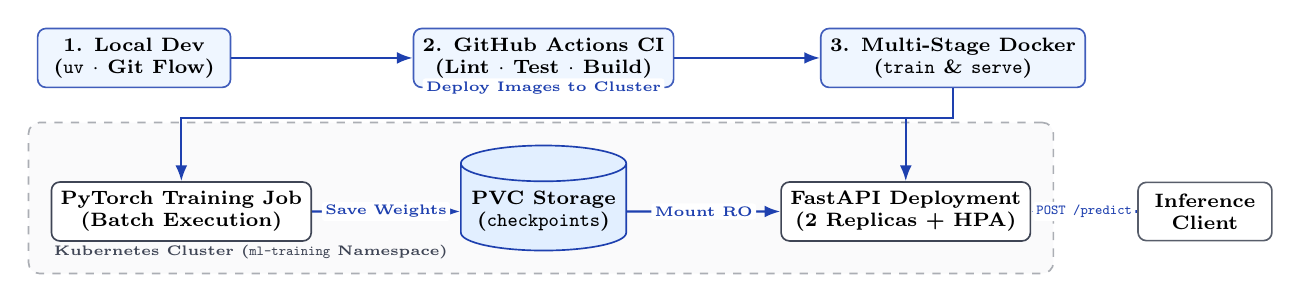
\begin{tikzpicture}[
    box/.style={rectangle, draw=deepblue!85, fill=softblue, rounded corners=3pt, minimum width=2.45cm, minimum height=0.74cm, align=center, font=\scriptsize\bfseries, line width=0.6pt},
    k8snode/.style={rectangle, draw=primarydark!80, fill=white, rounded corners=3pt, minimum width=2.3cm, minimum height=0.74cm, align=center, font=\scriptsize\bfseries, line width=0.6pt},
    vol/.style={cylinder, shape border rotate=90, draw=deepblue, fill=borderblue!45, aspect=0.22, minimum width=2.1cm, minimum height=0.74cm, align=center, font=\scriptsize\bfseries, line width=0.6pt},
    arrow/.style={-{Latex[length=2.0mm]}, thick, color=deepblue},
    lbl/.style={font=\tiny\bfseries, text=deepblue, fill=white, inner sep=1.2pt, rounded corners=1pt}
]
    % --- Level 1: CI/CD & Build Pipeline ---
    \node[box] (dev) at (0, 0) {1. Local Dev\\(\texttt{uv} $\cdot$ Git Flow)};
    \node[box] (ci) at (5.2, 0) {2. GitHub Actions CI\\(Lint $\cdot$ Test $\cdot$ Build)};
    \node[box] (docker) at (10.4, 0) {3. Multi-Stage Docker\\(\texttt{train} \& \texttt{serve})};

    % --- Level 2: Kubernetes Orchestration ---
    \node[k8snode] (job) at (0.6, -1.95) {PyTorch Training Job\\(Batch Execution)};
    \node[vol] (pvc) at (5.2, -1.95) {PVC Storage\\(\texttt{checkpoints})};
    \node[k8snode] (serve) at (9.8, -1.95) {FastAPI Deployment\\(2 Replicas + HPA)};
    \node[box, fill=white, draw=primarydark!70, minimum width=1.7cm] (client) at (13.6, -1.95) {Inference\\Client};

    % Connections Level 1
    \draw[arrow] (dev) -- (ci);
    \draw[arrow] (ci) -- (docker);

    % Connections Level 1 -> Level 2
    \draw[arrow] (docker.south) -- ++(0,-0.38) -| (job.north);
    \draw[arrow] (docker.south) -- ++(0,-0.38) -| (serve.north);
    \node[lbl, text=deepblue] at (5.2, -0.38) {Deploy Images to Cluster};

    % Connections Level 2
    \draw[arrow] (job) -- node[lbl]{Save Weights} (pvc);
    \draw[arrow] (pvc) -- node[lbl]{Mount RO} (serve);
    \draw[arrow] (client) -- node[lbl]{\texttt{POST /predict}} (serve);

    % K8s Boundary Box
    \begin{scope}[on background layer]
        \node[draw=primarydark!35, fill=primarydark!2, rounded corners=4pt, dashed, line width=0.6pt,
              fit=(job) (pvc) (serve), inner xsep=8pt, inner ysep=8pt,
              label={[anchor=south west, font=\tiny\bfseries\color{primarydark!80}, xshift=6pt, yshift=2pt]south west:Kubernetes Cluster (\texttt{ml-training} Namespace)}] {};
    \end{scope}
\end{tikzpicture}
\end{center}
\vspace{1pt}

% --- Git Workflow & Pull Requests ---
\section{Git Workflow \& Pull Requests}

This repository strictly adheres to the Git Flow branching model and the \textbf{\href{https://www.conventionalcommits.org/}{Conventional Commits}} specification:
\begin{itemize}[leftmargin=1.5em]
    \item \textbf{\texttt{main}}: Production release branch.
    \item \textbf{\texttt{develop}}: Primary integration branch.
    \item \textbf{\texttt{feature/*}}: Isolated feature branches merged via reviewed Pull Requests with structured changelogs.
\end{itemize}

\subsection{Pull Requests Summary}

\begin{table}[H]
\centering
\small
\begin{tabularx}{\textwidth}{@{} l >{\raggedright\arraybackslash}p{4.2cm} X c @{}}
\toprule
\textbf{PR} & \textbf{Branch Target} & \textbf{Key Implementations \& Deliverables} & \textbf{Status} \\
\midrule
\href{https://github.com/risan-raja/mlops-pytorch-pipeline/pull/1}{\textbf{PR \#1}} &
\texttt{feature/requirements} $\rightarrow$ \texttt{develop} &
Setup Astral \texttt{uv} package management, \texttt{pyproject.toml}, lockfiles, and CPU-only PyTorch indexes. &
\textcolor{taggreen}{\textbf{Merged}} \\
\addlinespace[2pt]
\href{https://github.com/risan-raja/mlops-pytorch-pipeline/pull/2}{\textbf{PR \#2}} &
\texttt{feature/ci} $\rightarrow$ \texttt{develop} &
Added GitHub Actions CI pipeline with Ruff linting, Pyrefly type checking, pytest unit tests, and Docker validation. &
\textcolor{taggreen}{\textbf{Merged}} \\
\addlinespace[2pt]
\href{https://github.com/risan-raja/mlops-pytorch-pipeline/pull/3}{\textbf{PR \#3}} &
\texttt{feature/modelling} $\rightarrow$ \texttt{develop} &
Implemented PyTorch CNN model, CIFAR-10 data loaders, training loop with JSON metrics, and FastAPI serving. &
\textcolor{taggreen}{\textbf{Merged}} \\
\addlinespace[2pt]
\href{https://github.com/risan-raja/mlops-pytorch-pipeline/pull/4}{\textbf{PR \#4}} &
\texttt{feat/kubernetes} $\rightarrow$ \texttt{develop} &
Implemented multi-stage Dockerfiles, Kubernetes Job, persistent storage claims, autoscaled Deployments, and probes. &
\textcolor{taggreen}{\textbf{Merged}} \\
\addlinespace[2pt]
\href{https://github.com/risan-raja/mlops-pytorch-pipeline/pull/5}{\textbf{PR \#5}} &
\texttt{develop} $\rightarrow$ \texttt{main} &
Consolidated production release merging all tested infrastructure, automation scripts, and documentation. &
\textcolor{taggreen}{\textbf{Merged}} \\
\bottomrule
\end{tabularx}
\caption{Summary of Git Flow Pull Requests and integration deliverables.}
\label{tab:prs}
\end{table}

\newpage

% --- Reflection & Technical Analysis ---
\section{Reflection \& Technical Analysis}

\begin{reflectionbox}{1. What was the most difficult part of this project?}
The most difficult portion of developing this pipeline was managing \textbf{persistence of data in Kubernetes asynchronous Job streams}, as well as \textbf{containerized storage provisioning}:
\begin{itemize}[leftmargin=1.3em]
    \item \textbf{Compatibility between storage class access modes and provisioning for local containers}: The local provisioners for Kubernetes (for example Docker Desktop / Rancher \texttt{local-path}) can only provide a \texttt{ReadWriteOnce} access mode. Distributed clusters utilize cloud-based or NFS file systems that provide a \texttt{ReadWriteMany} access mode. Creating a checkpoint persistent volume claim that was writable by the batch Job and subsequently read-only mounted by the serving deployment required managing both the storage life cycle and isolation.
    \item \textbf{Probing timings \& cold starts}: During initialization, the container loads the PyTorch model weights from disk into memory. By tuning \texttt{initialDelaySeconds} (15 seconds) and \texttt{periodSeconds} on the Readiness Probe, we could prevent Kubernetes from routing user-inference requests to uninitialized containers during the initial cold-start process.
\end{itemize}
\end{reflectionbox}

\vspace{3pt}

\begin{reflectionbox}{2. Using Astral's \texttt{uv} in a Multi-Stage Build to Improve Dependencies}
Utilizing Astral's \texttt{uv} within our Docker multi-stage builds (\texttt{ghcr.io/astral-sh/uv} builder + \texttt{python:3.13-slim} runtime) greatly improved our build speeds and allowed us to take advantage of Docker's layer caching. We configured an explicit PyTorch-cpu wheel index to preclude the need for multi-gigabyte CUDA binaries to bloat our image size and keep the final serving container lightweight and fast to start.
\end{reflectionbox}

\vspace{3pt}

% --- Summary & Verification Matrix ---
\section{Summary of Pipeline Manifests \& Components}

\begin{table}[H]
\centering
\small
\begin{tabularx}{\textwidth}{@{} l l X @{}}
\toprule
\textbf{Layer} & \textbf{File / Manifest} & \textbf{Operational Role} \\
\midrule
\textbf{Configuration} & \texttt{configs/training\_config.yaml} & Declarative hyperparameters (LR, batch size, epochs, early stopping). \\
\addlinespace[1.5pt]
\textbf{Containers} & \texttt{docker/Dockerfile.train} & Multi-stage PyTorch training image with volume mount points. \\
& \texttt{docker/Dockerfile.serve} & Non-root lightweight inference container running FastAPI on port 8080. \\
\addlinespace[1.5pt]
\textbf{Kubernetes} & \texttt{k8s/namespace.yaml} & Dedicated \texttt{ml-training} namespace for isolated workloads. \\
& \texttt{k8s/configmap.yaml} & Declarative hyperparameters mounted to \texttt{/app/configs}. \\
& \texttt{k8s/pvc.yaml} & PersistentVolumeClaim for model weights persistence (\texttt{/app/checkpoints}). \\
& \texttt{k8s/training-job.yaml} & Batch training Job with CPU/Memory limits and GPU support readiness. \\
& \texttt{k8s/serving-deployment.yaml} & 2-replica serving Deployment with Readiness and Liveness probes. \\
& \texttt{k8s/serving-service.yaml} & ClusterIP Service routing cluster port 80 to container port 8080. \\
& \texttt{k8s/hpa.yaml} & Horizontal Pod Autoscaler targeting 70\% CPU utilization. \\
\bottomrule
\end{tabularx}
\caption{Key configuration manifests, container definitions, and deployment artifacts.}
\label{tab:manifests}
\end{table}

\end{document}
